%-------------------------------------------------
% CVL Technical Report
% Author: Markus Diem
% Date: 05.07.2010
% Affiliation:
%		Vienna University of Technology
%		Faculty of Informatics
%		Institute of Computer Aided Automation
% 	Computer Vision Lab
%-------------------------------------------------
\documentclass[12pt,a4paper]{article}

% include packages ---------------------------------------------------

%\usepackage[ngerman]{babel}			% uncomment if you write it in german

\usepackage[pdfborder=0]{hyperref}	% links without border
%\usepackage{url}										% uncomment if hyperref is commented
%\linespread{1.2}										% use this for a short report :)

\usepackage{amsmath}
\usepackage{graphicx}
\usepackage[noindentafter]{titlesec}
% \usepackage[ansinew]{inputenc}      % ---> f�r umlaute in deutschen references
\usepackage[utf8]{inputenc}
\usepackage[T1]{fontenc} 
\usepackage[printonlyused]{acronym}	% acronyms
\usepackage{changepage}							% for the titlepage
\usepackage{a4}											% margin

\usepackage{listings}
\usepackage{xcolor}
\colorlet{punct}{red!60!black}
\definecolor{background}{HTML}{EEEEEE}
\definecolor{delim}{RGB}{20,105,176}
\colorlet{numb}{magenta!60!black}

\lstdefinelanguage{json}{
    numbers=left,
    numberstyle=\scriptsize,
    stepnumber=1,
    showstringspaces=false,
    breaklines=true,
    frame=lines,
    literate=
     *{0}{{{\color{numb}0}}}{1}
      {1}{{{\color{numb}1}}}{1}
      {2}{{{\color{numb}2}}}{1}
      {3}{{{\color{numb}3}}}{1}
      {4}{{{\color{numb}4}}}{1}
      {5}{{{\color{numb}5}}}{1}
      {6}{{{\color{numb}6}}}{1}
      {7}{{{\color{numb}7}}}{1}
      {8}{{{\color{numb}8}}}{1}
      {9}{{{\color{numb}9}}}{1}
      {:}{{{\color{punct}{:}}}}{1}
      {,}{{{\color{punct}{,}}}}{1}
      {\{}{{{\color{delim}{\{}}}}{1}
      {\}}{{{\color{delim}{\}}}}}{1}
      {[}{{{\color{delim}{[}}}}{1}
      {]}{{{\color{delim}{]}}}}{1},
}

\usepackage{url}

% our style
% creates the titlepage & does all the formating
\usepackage{cvl-titlepage}


% ------------------------------------------------
%	How to make LaTeX copy & paste -able for WORD (final spell checking):
%	- uncomment the subsequent commands so that
%   fi and ff are correct symbols
% - comment hyperref & uncomment url
%	- copy & paste the *.pdf text
% - In word: replace (ctrl+H) ^p with a whitespace
%   this removes paragraph breaks
% - the subsequent commands surpress ligatures & page numbering
%\usepackage{microtype}
%\DisableLigatures{encoding = *, family = * }
%\pagestyle{empty}
% ------------------------------------------------

% hyphenation
\hyphenation{kle-ber}


% title information -----------------------------------------------
\title{Online Medical Imaging Platform}
\author{Willinger Christin}
\newcommand{\supervisor}{Robert Sablatnig}
%\newcommand{\subsupervisor}{Sebastian Zambanini}	% uncomment if you have two supervisors

%\date{July 5, 2010}	% use this if you need a specific date

% title information -----------------------------------------------

% readme ----------------------------------------------------------
% Some hints...
% - do not make a tableofcontents
% - the proposed structure (introduction, related work, ...)
% - if you have any questions concerning latex, or the proposed
%   style sheet, contact your supervisor.
% - if you detect errors within this style sheet, contact: 
%		diem@caa.tuwien.ac.at
% - please keep the abstract short enough to fit on the title page
% - concentrate on the essential content, but do not write bushwa
% 	in order to extend your thesis
% - do not use filler words such as: much, more, many...
% - do not write statements with out proof such as:
%   Recently, document analysis has become an important field.
% - don't ever cite wikipedia
% - but you should cite all papers, your work is based upon
% - if you chose a specific method, always state the reason
% - some general hints for literature research:
% 		- http://dblp.mpi-inf.mpg.de/dblp-mirror/index.php
% 			the webpage may seem old-fashioned, but it has 
% 			a live search and indexes all important conferences
% 			(not solely IEEE or ACM...). additionally links to 
% 			the bibtex and the *.pdf are provided
% 		- http://ieeexplore.ieee.org/Xplore/dynhome.jsp
% 			the official IEEE search engine (you need a TU VPN
% 			in order to access the *.pdfs)
%			- http://portal.acm.org/portal.cfm
% 			crappy, but the official acm search engine
% 		- http://jabref.sourceforge.net/
% 			nice tool to organize your references
% 		- http://www.citeulike.org/
% 			some people think it is best...
% - if you are bored while writing: 
%   http://stud3.tuwien.ac.at/~e0226595/james-bomb/index.htm
% readme ----------------------------------------------------------

\begin{document}

\maketitlepage
\pagenumbering{roman}
\tableofcontents
% put your abstract here
\abstract{
}
\clearpage
\pagenumbering{arabic}

%----------------------------------------------
% Introduction
%----------------------------------------------
\section{Introduction}
\label{sec:introduction}

%----------------------------------------------
% * Motivation 
%----------------------------------------------
\subsection{Motivation}
\label{sec:Motivation}

%----------------------------------------------
% ** Interaktion mit einer Bildsuchmaschiene
%----------------------------------------------
\subsubsection{Interface für Kreshmoi}
\label{sec:Interface für Kreshmoi}
Das Ziel von KHRESMOI ist das Durchsuchen und der Zugang zu medizinischen Informationen für verschiedene Benutzergruppen mit unterschiedlichem medizinischen Vorwissen.
Die Einteilung der Benutzer erfolgt in 3 Kategorien:
\begin{itemize}
	\item Personen ohne speziellen medizinischen Kentnissen
	\item Ärzte
	\item Radiologen
\end{itemize}
Dazu verknüpft KHRESMOI Daten aus verschiedenen heterogenen Resourcen wie Bildern aus PACS, Bildern und Text aus Publikationen in Journalen oder Daten von Webseiten.
Da sich die verschiedenen Resoucen qualitativ sehr stark voneinander unterscheiden können wird einen Bewertung ihrer Glaubwürdigkeit durchgeführt und dem Benutzer angezeigt.
\\
Die Suchanfrage kann in textueller Form oder als Bild-Query sowie als Kombination von beidem gestellt werden.
Ein weiteres wichtiges Feature hiebei ist die multilinguale Suche, da die Menge an verfügbaren medizinischen Informationen nicht in alle Sprachen gleich ist.
Dies bedeutet dass die Suchanfrage in mehrere Sprachen übersetzt wird und somit auch anderssprachige Quellen durchsucht werden können.
Die Zusammenfassungen der Suchergebnisse werden anschließend in die Anfragesprache rückübersetzt wodurch der Benutzer schnell duch die Ergebnissliste navigieren kann.

%----------------------------------------------
% ** Interaktion mit einer Bildsuchmaschiene
%----------------------------------------------
\subsubsection{Interaktion mit einer Bildsuchmaschiene}
\label{sec:Interaktion mit einer Bildsuchmaschiene}
Ein Teilprojekt von KHRESHMOI ist das Druchsuchen von medizinischen Bilddaten wobei diese in 2D, 3D oder 4D (Video) vorliegen können.
Um eine Suchanfrage auf ein Bild stellen zu können müssen an einem Referenz-Bild Bereiche eingezeichnet werden welche dann die Anfrage formen.
Aus der Textur eines markierten Bereiches wird ein Feature-Vektor extrahiert mit dem anschließend eine Datenbank von zuvor indizierten Bildern durchsucht wird.
\\
Ein Frontend einer Bildsuchmaschiene muss daher sowohl Tools zum markieren von interessanten Bereichen, 
als auch die Funktionalität zur verfnünftigen Berachtung der Bilder bereitstellen.
\\
Diese Arbeit spezialisiert sich auf das Durchsuchen von radioloischen Aufnahmen in 2D und 3D welche in einem PACS (Picture Archiving and Communication Systems) abgelegt sind.
Da in einem Krankenhaus täglich große Mengen an Daten durch radionlogische Aufnahmen produziert werden, 
bietet eine effizientes Durchsuchen dieser die möglichkeit Sie für Ausbildung und Forschug wieder zu verwenden.
\\
Dazu muss das User-Interface die grundliegenden Funktionen eines Betrachtungs-Tools für Röngten- und Computertomographie-Aufnahmen zur verfüfung Stellen:
\begin{itemize}
	\item Zoom
	\item Schnelles anpassen von Kontrast und Helligkeit
	\item Navigation durch die Schnitte eins 3D-Körpers in einer Schnittachse
\end{itemize}


%----------------------------------------------
% * Pflichtenheft
%----------------------------------------------
\subsection{Pflichtenheft}
\label{sec:Pflichtenheft}
\begin{itemize}
	\item Kommunikation mit KRESHMOI über HTTP Anfragen. Dies beinhaltet das Senden von Suchanfragen, auswerten der Ergebnisse und laden der zugehörigen Bilder.
	\item Betrachen von CT Volumes. Navigation durch die einzelnen Schnitte eines Volumes entlang einer auswählbaren Achse.
	\item Schnelles anpassen von Kontrast und Helligkeit bei den einzelnen Schnittbildern mit der Maus (Fensterung).
	\item Zoomen und Scrollen des Bildausschnittes in einem Bild oder Volume.
	\item Tools zum Anotieren von Bereichen innerhalb der Bildern welche zur Interaktion mit der Bildsuche dienen.
	\item Präsentation der Suchergebnisse.
	\item Anzeige der den Bildern oder Volumes zugehörigen Reports.
	\item Ansicht zum vergleichen von verschiedenen Ergebnissen.
	\item Modulare Komposition der verschidenen Ansichten.
	\item Umsetzung der Applikation im Webbrowser.
\end{itemize}

%----------------------------------------------
% * Möglichkeiten zu Umsetzung
%----------------------------------------------
\subsection{Möglichkeiten zur Umsetzung}
\label{sec:Möglichkeiten zur Umsetzung}
Aufgrund der Anforderung dass, das Programm in einem Webbrowser ausgeführter werden soll, gibt es zwei Möglichkeiten die Anwendung umzusetzen.

%----------------------------------------------
% ** JavaApplet
%----------------------------------------------
\subsubsection{JavaApplet}
\label{sec:JavaApplet}
Bei einem Java Applet wird ein Java Programm in eine Webseite eingebunden und vom dem Browser des Clients geladen.
Der Browser übergibt das Applet dem Java Interpreter wofür aber ein spezieller Plugin notwendig ist.
\\
Der große Vorteil dieses Ansatzes ist dass die Anwendung sehr performant ist.
Dies ergibt aus den beiden Punkten dass Java Code compiliert wird und dass es möglicht ist die Grafikhardware des Clients zum bearbeiten der Bilder zu verwenden,
welche für diese Aufgabe besser geeignet ist als die CPU.
\\
Dafür müssen die notwendigen Plugins sowie ein aktueller Java Interpreter auf dem Client installiert sein, 
was bei manchen Betriebssystemen für Mobiledevices gar nicht möglich ist.
%----------------------------------------------
% ** HTML5
%----------------------------------------------
\subsubsection{HTML5}
\label{sec:HTML5}
Bei deisem Ansatz wird die Anwendung in HTML, CSS und JavaScript oder einem Framework welches auf diesen Technologien aufsetzt entwickelt.
\\
Da diese Technologien von fast allen neuen Browsern unterstütz werden kann damit ein sehr hoher Grad an Portabilität erreicht werden.
Weiters sind Webapplikationen für den Benutzer sehr einfach zu verwenden da anstatt einer Installation um die Anwendung nutzen zu können nur eine Webseite geöffnet werden muss.
\\
HTML5 unterstüzt Canvas Elemente für 2D Bilder jedoch ist eine Verarbeitung der Bilder durch die Grafikhardware nur begrenzt möglich.
Für die Verwendung der Grafikarte durch den Browser gibt es die Schnittstelle WebGL welche auf OpenGL ES aufbaut.
Diese wurde aber noch nicht in allen gängigen Browsern implementiert bzw ist in einigen nocht nicht stabil und muss extra aktiviert werden.





%!TEX root = cvl_bachelor_thesis.tex

%----------------------------------------------
% Related Work
%----------------------------------------------
\section{Related Work}
\label{sec:relatedWork}
Software für die Bildsuche in radiologischen Daten gibt es bis jetzt noch nicht,  
allerdings decken sich die Anforderungen großteils mit Betrachtungstools für 2D und 3D Daten aus der Radiologie und Nuklearmedizin.
Solche Softwareprodukte finden sich in den Betrachtungs-Workstations von PACS-System in Krankenhäusern oder als Betrachtungstools für Datensätze des offenen Standards DICOM.
Die beiden Konzepte PACS und DICOM werden im folgenden Kapitel kurz erklärt, sowie die Umsetzung der benötigten Funktionalität in zwei konkreten Softwareprodukten diskutiert.

%----------------------------------------------
% * PACS-Systeme
%----------------------------------------------
\subsection{PACS-Systeme}
\label{sec:PACS-Systeme}
Ein PACS-System (Picture Archiving and Communication System) dient zum Speichern und Austausch von medizinischen Bilddaten.
Obwohl es prinzipiell für alle bildgebenden Verfahren verwendet werden kann,
wird es vorwiegend für Daten aus der Radiologie und Nuklearmedizin genutzt.
%
Das Systems setzt sich aus dem PACS Server und den Workstations zusammen.
Der Server sammelt Daten von den bildgebenden Geräten,
 verknüpft Sie mit Daten aus einem Krankenhaus Informations System (KIS) oder Radiologie Informations System (RIS) und sorgt für ihre Archivierung in einem Kurz- oder Langzeitarchiv. 
Die Kommunikation mit den bildgebenden Geräten erfolgt meist durch ein Protokoll welches den DICOM Standard implementiert.
%
Die Befundung erfolgt auf den PACS Workstations welche die Daten vom Server laden und anzeigen.
Die Workstation stellte die Funktionalität zur Betrachtung und zum Nachbearbeiten der Bilder zur Verfügung.
Änderungen der Daten werden von der Workstation zurück auf den Server geladen.
Je nach Funktionsumfang stehen auch Tools zur Befundung zur Verfügung welche die Daten an das RIS oder KIS weiter geben \cite{pacs}.

%----------------------------------------------
% * DICOM
%----------------------------------------------
\subsection{DICOM}
\label{sec:DICOM}
DICOM steht für \emph{Digital Imaging and Communication in Medicine} und ist ein offener,
Standard welcher die Übertragung und das Speichern von medizinischer Bildinformation spezifiziert.
Die wesentlichen Teile der Spezifikation sind die Datenstruktur für die Bilddaten und \C{zugehörige Informationen wie Patientendaten oder Daten über das Aufnahmegerät} , 
Services welche auf diesen Daten operieren, Anforderung an DICOM konforme Hard- und Software-Produkte und das Ablegen der Informationen auf einem Datenträger.
Das Datenmodell setzt sich in Anlehnung an die reale Welt grundlegend aus den Entitäten Patient, Studie, Serie und Image zusammen zwischen denen jeweils eine 1:n oder 0:n Beziehung besteht.
Es bietet weiters ausreichend Möglichkeiten zur Erweiterung durch einen Definitionsmechnanissmus für alle DICOM Objekte die sogenannte Image Object Defintion \cite{pacs}.

%----------------------------------------------
% * Osirix
%----------------------------------------------
\subsection{Osirix}
\label{sec:Osirix}
OsiriX ist eine Software zur Betrachtung und Nachbearbeitung von DICOM Bilddaten.
Sie wird als freie Open-Source-Software unter der GPL für das Betriebssystem Mac OS X entwickelt.
OsiriX ist nur für die Forschung und dem privaten Gebrauch zugelassen, 
für einen diagnostischen Einsatz in der Medizin steht die kostenpflichtige Version OsiriX MD zur Verfügung.
%
Das Programm führt eine Datenbank von DICOM Datensätzen, 
welche von DICOM-Dateien importiert bzw. auch wieder als solche exportiert werden können.
Weiters können über das DICOM-Protokoll die Daten auch von einem PACS-Server geladen werden \cite{osirix}.

Von der Navigationsstruktur unterteilt sich OsiriX in eine Datenbankebene \ref{fig:osirix_db_view} und eine Betrachtungsebene welche jeweils durch verschiedene Fenster umgesetzt wurden.
Der Vollständigkeit halber sei erwähnt das es auch eine Ebene für 3D Rendering der Volumes gibt welche aber für diese Arbeit nicht relevant ist.
\begin{figure}[t]
	\centering
	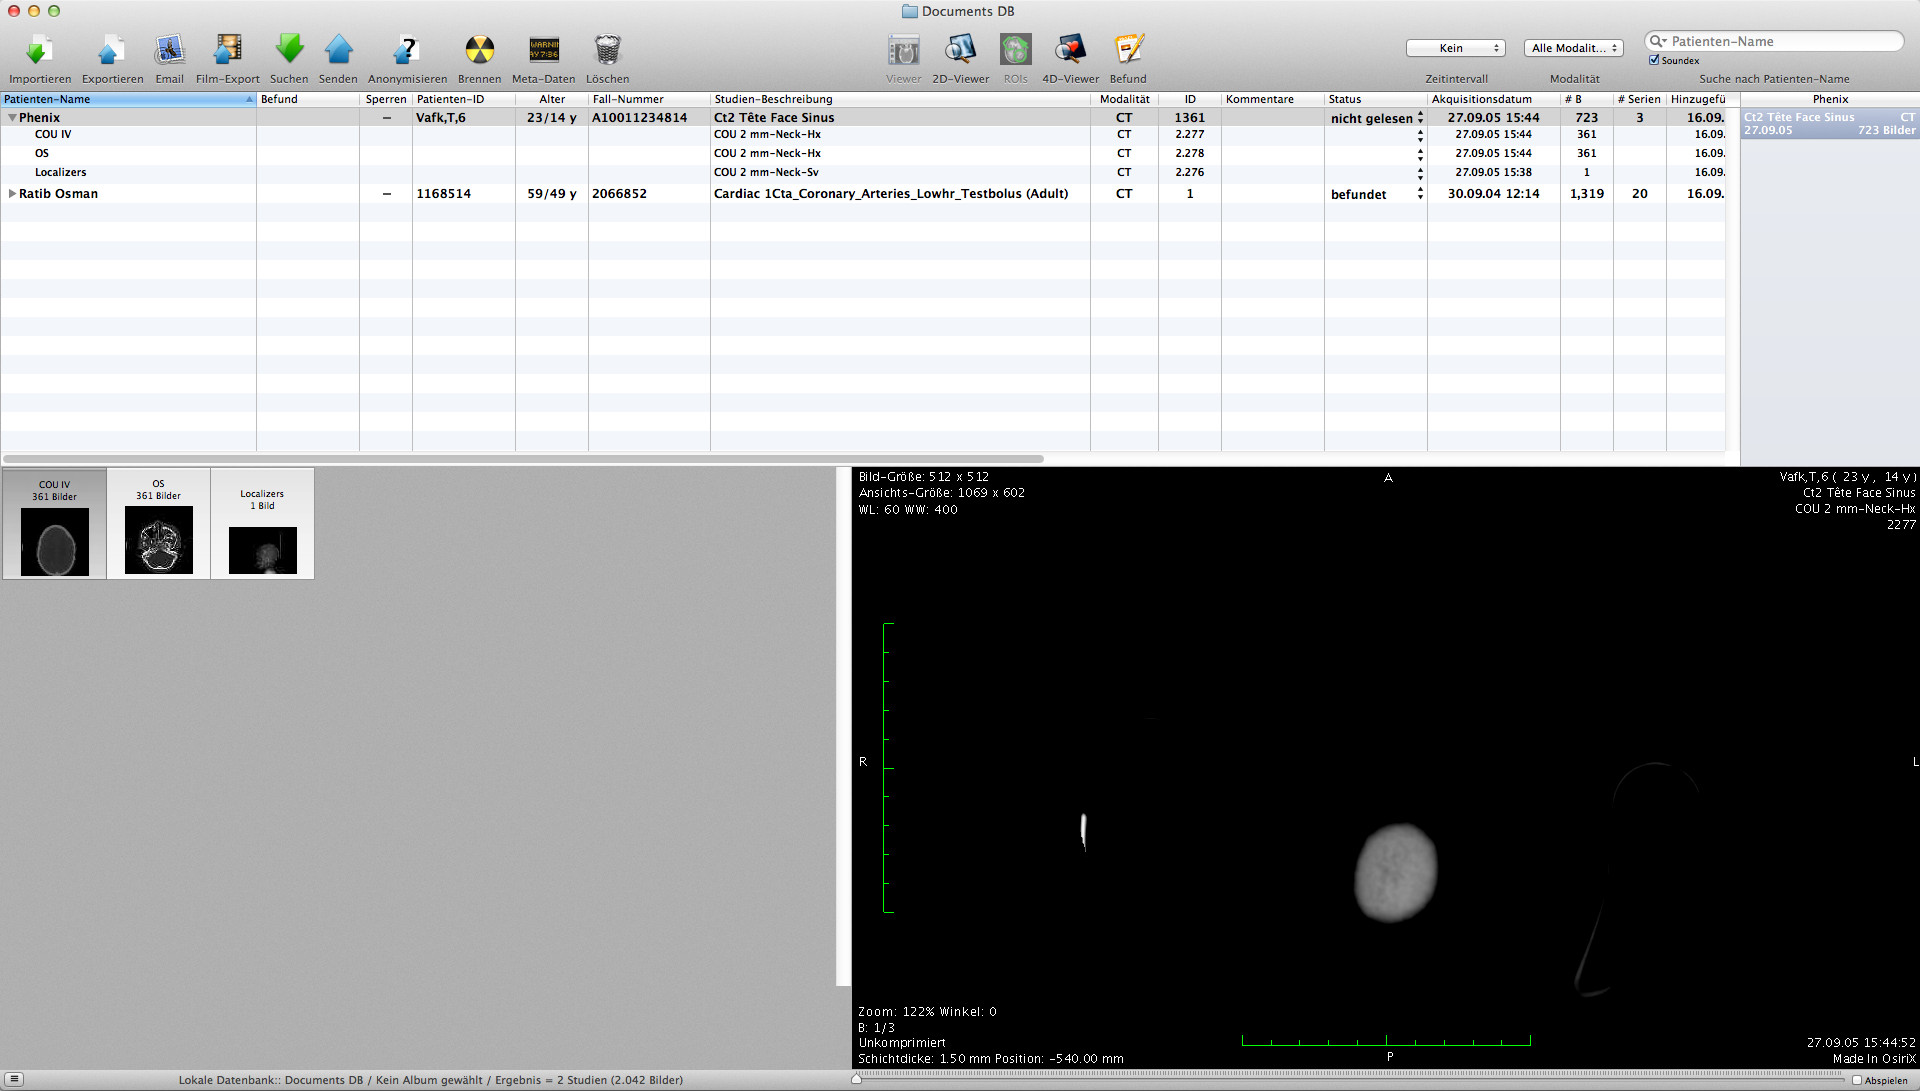
\includegraphics[width=0.8\linewidth]{img/c2_osirix_db_view.jpg}
	\caption{Datenbankansicht von OsiriX.}
	\label{fig:osirix_db_view}
\end{figure}
In der Datenbankebene können die Datensätze importiert, exportiert und durchsucht werden, wobei jede Studie für einen Patienten einen Eintrag in der Liste darstellt.
Weiters stehen Unterlisten zum Anzeigen der Serien einer Studie zur Verfügung.
Unter der Listenansicht werden die ausgewählten Einträge als Thumbnails und in einem minimalen 2D Betrachter,
welche die wichtigsten Funktionen der Betrachtungsebene implementiert, zur Vorschau dargestellt.
In der Betrachtungsebene \ref{fig:osiri_2dView_toolbar} \ref{fig:osirix_2dView_splitWindow} finden sich die eigentlichen Funktionen und Tools welche für die Interaktion mit den Bildern notwendig sind.
Dafür bietet OsiriX eine große Funktionspalette, wobei hier nur auf die Kernfunktionalität eingegangen wird \cite{osirix}.
\paragraph{Funktionsumfang}
Die Steuerung für die Tools zur Interaktion mit dem Volume erfolgt mit der Maus, 
welcher die spezifischen Funktionen zugewiesen werden können. Die jeweils zugewiesene Funktion wird durch das Drücken der Maustaste aktiv.
\begin{itemize}
	\item Bei der \textbf{Fensterung} wird mit der X-Achse wird die Fensterbreite (Kontrast) und mit der Y-Achse das Fensterzentrum (Helligkeit) angepasst.
	\item \textbf{Positionierung} des Bildes innerhalb der Anzeigefläche. Geht das Bild über die Anzeigefläche hinaus wird dies durch einen farbige Linie an der jeweiligen Kante signalisiert.
	\item \textbf{Zoom} durch das Verschieben der Maus entlang einer Achse.
	\item \textbf{Rotation} um das Bildzentrum durch das Verschieben  der Maus entlang der X-Achse.
	\item \textbf{Navigation} durch das Volume. Die Achse in der die Maus nach einem Klick zuerst verschoben wird, wird für die Navigation gewählt, die andere bleibt inaktiv.
	\item Einzeichnen von \textbf{ROIs}. Hierbei werden Punkte, Linien, Polygone, Winkel und noch weitere Geometrien unterstützt. 
		Sind in dem Datensatz die notwendigen Informationen vorhanden erfolgt einen automatische Vermessung der ROIs.
\end{itemize}
\begin{figure}[t]
	\centering
	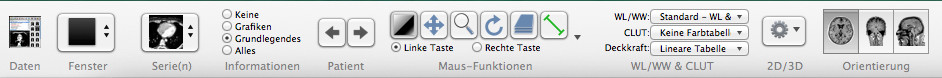
\includegraphics[width=0.8\linewidth]{img/c2_osirix_2d_view_toolbar.jpg}
	\caption{Toolbar für die 2D Batrachtungsebene.}
	\label{fig:osiri_2dView_toolbar}
\end{figure}
Weiters können mehrere Betrachtungs-Fenster nebeneinander angeordnet werden, wobei sich diese zur Darstellung unterschiedlicher Serien bzw. Orientierungen eines Datensatzes nutzen lassen. 
Die Orientierung gibt an entlang welcher Achse die Bilder eines Volumes geschnitten werden.
Wird in verschiedenen Fenstern eine unterschiedliche Orientierung gewählt,
so wird beim Navigieren durch das Volume in einem Fenster die Position der Schnittebene in den anderen als farbige Linie angezeigt \cite{osirix}.
\begin{figure}[t]
	\centering
	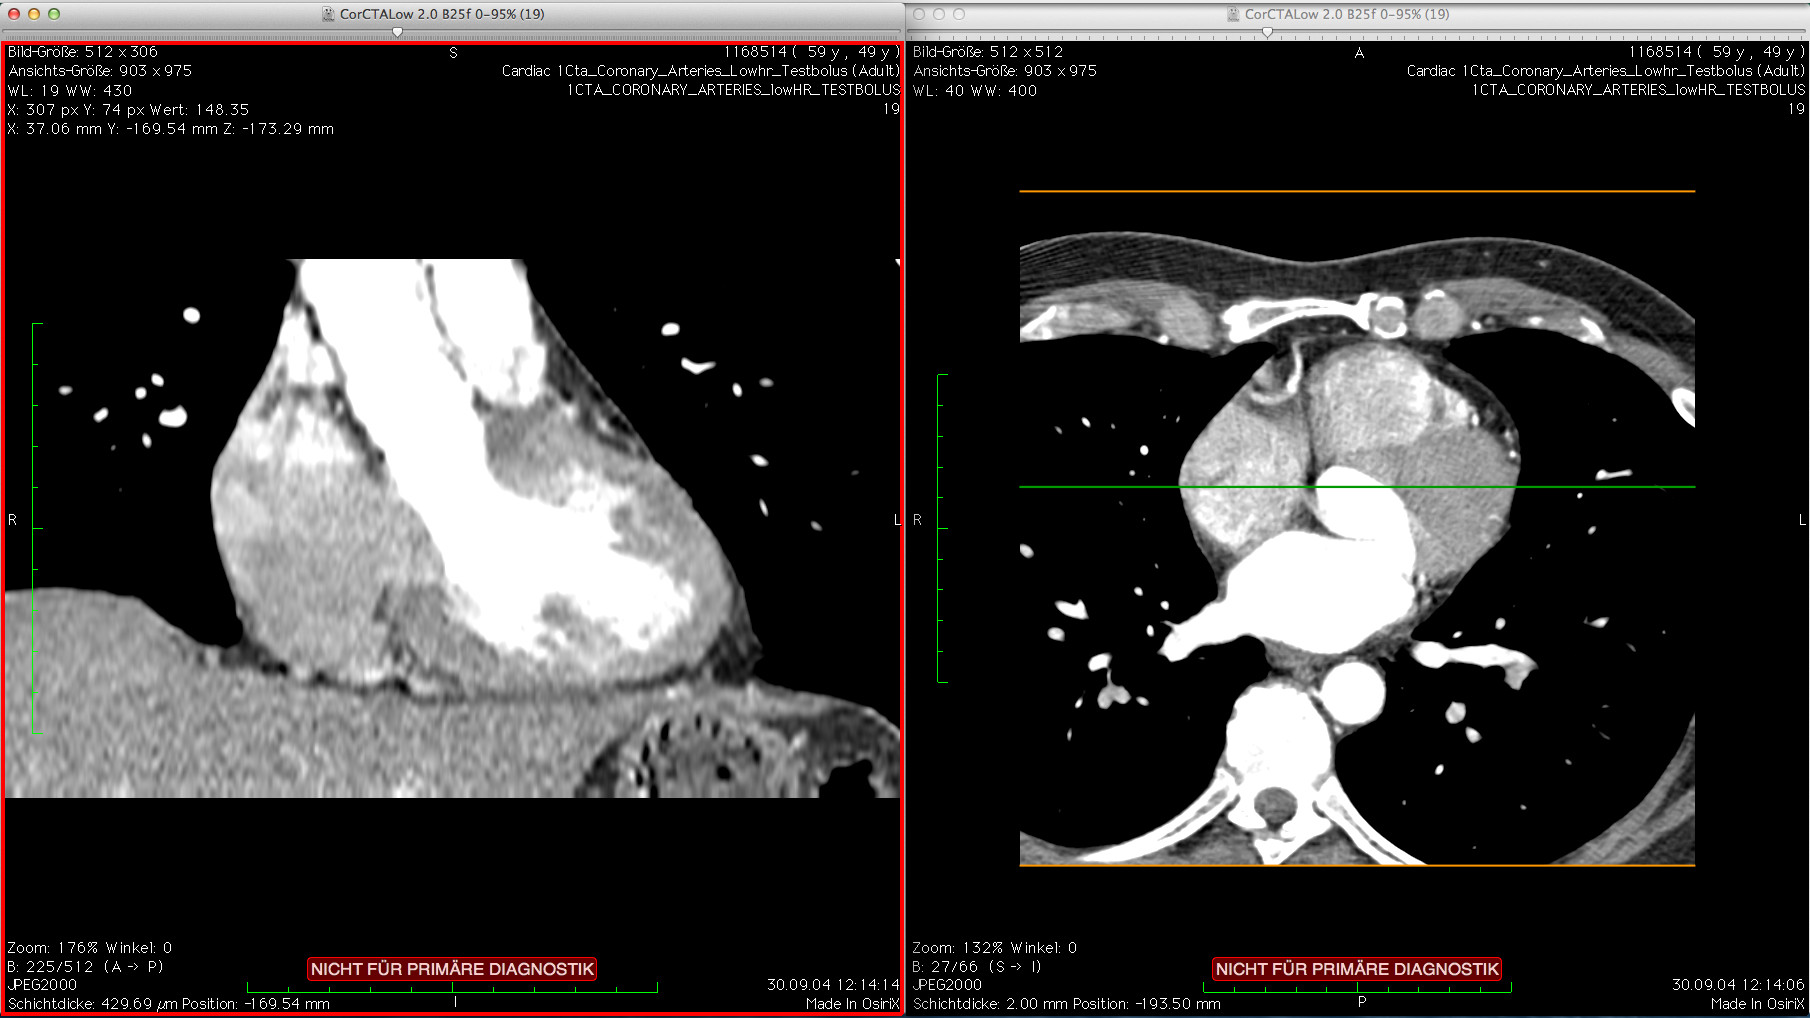
\includegraphics[width=0.8\linewidth]{img/c2_osirix_2d_view_splitscreen.jpg}
	\caption{Darstellung eines Volumes aus zwei verschiedenen Orientrierungen. Die Schnittposition des linken Bildes wird im rechten als grüne Linie dargestellt.}
	\label{fig:osirix_2dView_splitWindow}
\end{figure}

%----------------------------------------------
% * PACS Workstation - AFGA Impax DS3000
%----------------------------------------------
\subsection{PACS Workstation - AFGA Impax DS3000}
\label{sec:PACS_Workstation}
Die Impax DS3000 Radiologie Diagnosestation ist eine Client-Software für ein PACS System.
Der Aufbau der Software ist ähnlich wie bei OSIRIX \ref{sec:Osirix} in eine Ebene zum Durchsuchen der Datensätze und eine Betrachtungsebene \ref{fig:impacs_2d_view} unterteilt.
%
\begin{figure}[t]
	\centering
	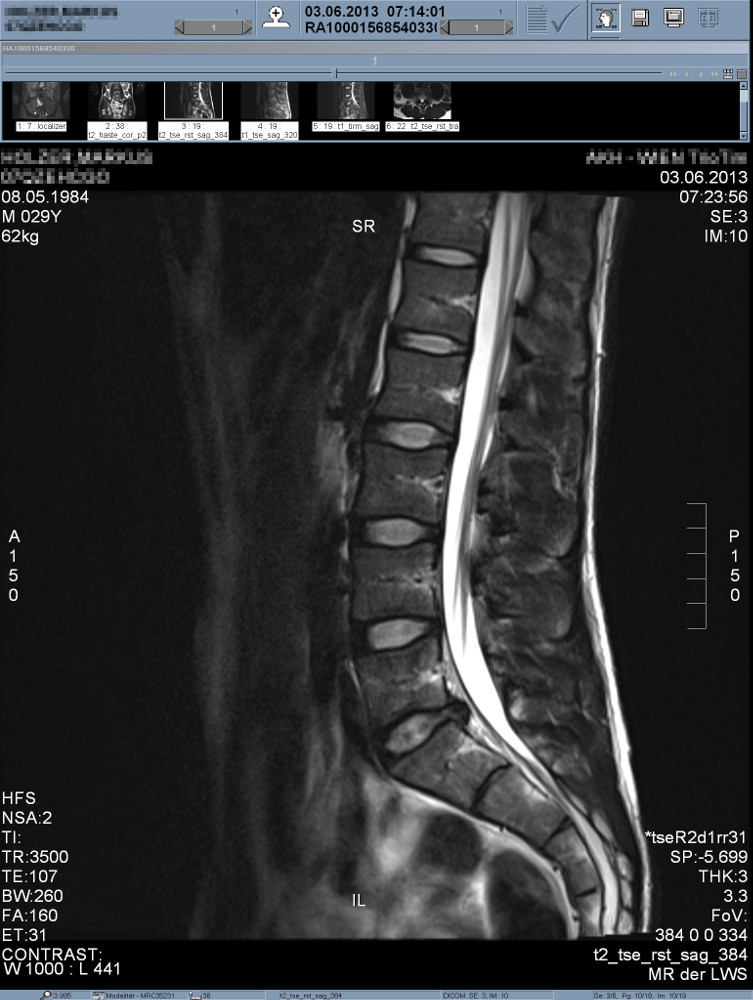
\includegraphics[width=0.5\linewidth]{img/c2_impacs_2d_view.jpg}
	\caption{Betrachtungsebene zum Anzeigen der Series}
	\label{fig:impacs_2d_view}
\end{figure}
%
Die Ebene für die Datensätze bietet Funktionen zum Durchsuchen von PACS Archiven anhand verschiedene Parameter wie Name, Patientenkennung oder Geburtsdatum.
Weiters können in dieser Ebene Arbeitslisten erstellt werden, in der sich die RadiologIn eine Menge von Fällen zum Befunden zusammenstellen kann.
Es gibt auch Tools zum automatischen Erstellen von Arbeitslisten anhand diverser Kriterien wie zum Beispiel alle CT-Aufnahmen des heutigen Tages.
%
Die Betrachtungsebene bietet mit den Tools für Fensterung, Positionierung, Zoom, Navigation im Volume und dem einzeichnen von ROIs die selbe Kernfunktionalität wie Osirix.
Auch bei Impax DS3000 werden diese Funktionen mit der Maus kontrolliert, deren Auswahl über ein Kontextmenu erfolgt welches mit der rechten Maustaste aktiviert wird.
Auch hier ist eine Aufteilung des Bildschirmes möglich um Bilder aus einer Serie oder aus verschiedenen Serien miteinander zu vergleichen.

%----------------------------------------------
% * Vergleich der Betrachtungstools
%----------------------------------------------
\subsection{Vergleich der Betrachtungstools}
\label{sec:Vergleich der Betrachtungstools}
Die Funktionen zur Interaktion mit den Bilddaten sind bei den beiden erwähnten Software-Produkten sehr ähnlich und auch annähernd gleich umgesetzt.
Osirix hat einige Features wie 3D-Rendering welche zwar für die Forschung interessant sind, für die medizinische Befundung aber größere keine Rolle spielen.
Funktionen zum Durchsuchen der Datensätze anhand einer Bild-Query weisen bei Produkte nicht auf.


%!TEX root = cvl_bachelor_thesis.tex

%-------------------------------------------------------
% Methodology
%-------------------------------------------------------
\section{Methodology}
\label{sec:methodology}

%----------------------------------------------
% * Verwendetet Technologien
%----------------------------------------------
\subsection{Verwendetet Technologien und Protokolle}
\label{sec:Verwendetet Technologien}
Bevor auf die eigentliche Umsetzung eingegangen wird werden die verwendeten Frameworks und Technologien dargestellt.
Ein Teil davon, wie HTTP und REST, wurden bereits durch das Interface für KRESHMOI festgelegt, 
ein weiterer ergab sich durch die Anforderung einer Web-Applikation.
Die Frameworks und Technologien für Grafik und GUI wurden gewählt weil mit ihnen eine schnelle Umsetzung der Anforderungen möglich war.

%----------------------------------------------
% ** HTTP
%----------------------------------------------
\subsubsection{HTTP}
\label{sec:HTTP}
HTTP (Hyper Text Transfer Protokoll) ist ein Protokoll zur Übertragung von Daten über ein Netzwerk welches auf TCP aufsetzt.
Der Datenaustausch zwischen zwei Kommunikationspartnern findet in der Form von Nachrichten statt, 
wobei der Client eine Anfrage an einen Server stellt und dieser die Anfrage bearbeitet und eine Antwort returniert.
%
Eine Nachricht setzt sich aus einem Header und einen Body zusammen.
Der Body enthält die Nutzdaten und der Header enthält Metadaten über die Nutzdaten.
Vom Aufbau der Nachricht unterscheiden sich Anfrage und Antwort nur in der ersten Zeile:
\begin{itemize}
	\item Anfrage: Enthält die HTTP-Methode, die URL welche auf die Resource am Server zeigt und die Protokollversion.
	\item Antwort: Enthält die Protokollversion und den Serverstatus. 
		Der Serverstatus liefert eine Aussage ob der Request erfolgreich bearbeitet wurde bzw welche Art von Fehler bei der Bearbeitung aufgetreten ist.
\end{itemize}
HTTP ist ein zustandsloses Protokoll, daher wird nach jeder Anfrage die Verbindung vom Server wieder abgebaut.
Für eine Zuordnung eines Clients muss dieser eine Session-ID mitsenden welche normalerweise im Header enthalten ist \cite{http}.

%--------------------------------------------- 
% ** REST
%----------------------------------------------
\subsubsection{REST}
\label{sec:HTTP}
REST ist im eigentlichen Sin\R{n} mehr ein Architektursti\Rd{e}l als ein Protokoll welcher mit HTTP umgesetzt wird.
Die Idee von REST ist\R{,} dass eine URL genau eine Ressource auf einem Server adressiert, 
wobei eine Ressource eine statische Datei oder das Ergebnis einer Aktion auf dem Server sein kann.
Dieser Architektursti\Rd{e}l lässt sich durch fünf Prinzipiell zusammenfassen \Rc{fix sentence}:
\begin{itemize}
	\item \textbf{Ressource mit eindeutiger Identifikation:}
		Jede Ressource wird durch eine URI (Uniform Resouce Identifier) weltweit eindeutig identifiziert.
		Diese adressiert unter anderem den Server auf den sich die Ressource befindet sowie Ressource auf dem Server selbst.
	\item \textbf{Hypermedia:}
		Verknüpfungen zu anderen Entitäten werden als Links auf die jeweiligen Ressourcen dargestellt.
		Weiters kann die Steuerung des Applikationszustandes durch Links auf weiter Aktionen durch Hypermedia umgesetzt werden.
	\item \textbf{Standard-Opperationen:}
		Es gibt ein definiertes Interface welches von jeder Ressource zur Verfügung gestellt werden muss.
		Dieses umfasst einen relativ kleinen Satz von Operationen welche auf die Ressource ausgeführt werden können.
	\item \textbf{Unterschiedliche Repräsentation der Resourcen:}
		Die Ressourcen können unterschiedliche Darstellungsformen haben.
		Ein Client kann also eine Ressource in einem bestimmten Format (z.B.: XML, HTML, JSON) anfordern,
		sofern diese Darstellung vom Server für die jeweilige Ressource unterstützt wird.
		In HTTP wird die gewünschte Darstellung im Header angegeben.
	\item \textbf{Zustandslose Kommunikation}
		Der Server hält keine Zustandsinformationen über den Client welche über die Dauer eines Requests hinaus gehen.
		Daher muss der Zustand einer Anwendung entweder am Client liegen oder vom Server in eine Ressource umgewandelt werden \cite{rest}. 
\end{itemize}


%----------------------------------------------
% ** JSON
%----------------------------------------------
\subsubsection{JSON}
\label{sec:JSON}
Bei JSON (JavaScript Object Notation) handelt es sich um ein Datenformat zum Austausch von Arrays und Objekt-Graphen.
JSON findet neben XML vor allem in der Kommunikation zwischen Client und Server bei Webanwendungen Verwendung, 
wobei JSON Daten wesentlich kompakter und damit ressourcensparender sind.
Wie bei XML werden Listen und Objekte in einer von Menschen lesbaren Form darstellt.
Dabei werden folgende Datentypen unterstützt\R{,} welche wiederum beliebig tief ineinander verschachtelt werden können: NULL, Boolean, Zahl, String, Array und Objekt \cite{ajax}.

%----------------------------------------------
% ** AJAX
%----------------------------------------------
\subsubsection{AJAX}
\label{sec:AJAX}
AJAX (Asynchronous JavaScript and XML) ermöglicht es einer Webanwendung\R{,} kleinere Mengen von Daten nachzuladen und damit Teile der Webseite dynamisch zu ändern, 
statt bei jeder Aktion die Webseite neu zu laden.
Benötigt die We\Rd{b A}\R{a}pplikation Daten vom Server\R{,} wird an diese\Rd{m}\R{n} eine HTTP Anfrage gesendet und Callback-Funktionen für den Fall einer Antwort oder eines Fehlers beim Browser registriert.
Erhält der Browser eine Antwort auf seine Anfrage ruft er die Callback-Funktion auf und übergibt die erhalten Daten\R{,} wodurch die Webanwendung mit der Verarbeitung dieser fortfahren kann.
Dies ermöglicht die Entwicklung komplexer Webapplikationen, 
wobei die Webapplikation selbst mit der Seite geladen wird und die Daten\R{,} die der Benutzer mit der Anwendung verarbeiten möchte\R{,} dynamisch von der Anwendung nachgeladen werden können \cite{ajax}.

%----------------------------------------------
% ** Objectiv J
%----------------------------------------------
\subsubsection{Objectiv J}
\label{sec:Objectiv J}

Objective J ist eine Programmiersprache welche sich von der Syntax stark an Objective\R{-}C anlehnt.
Sie ist eine Erweiterung oder Obermenge von Javascript und wird von einem in Javascript geschriebenen Interpreter abgearbeitet.
In Javascript können Objekte durch Prototyping erstellt werden, das Konzept von Klassen wird aber nicht unterstützt.
Obj\Rc{konsistente schreibweise} J bietet zusätzlich zu den nativen JS \Rd{abkuerzung nicht definitert, ausschreiben is eh besser.}Objekten die Definition von Klassen inklusive Vererbung und die Generierung von Objekten daraus.
Obwohl es die Sprache erlaubt für Variablen, Methodenparameter und Rückgabe einer Funktion eine\Rc{fix} Datentyp zu definieren, 
werden diese aufgrund von schwacher Typisierung vom Interpreter nicht auf ihre Einhaltung überprüft.
In der aktuellen Version wird die Übergabe von Referenzen als Parameter ähnlich einem Pointer in C unterstützt \cite{capp}.

%----------------------------------------------
% ** Cappuccino
%----------------------------------------------
\subsubsection{Cappuccino}
\label{sec:Cappuccino}
Bei Cappuccino handelt es sich um ein Web Application Framework für Objectiv\Rc{bindestrich }J und Javascript, welches hauptsächlich der Erstellung komplexer Benutzeroberflächen dient.
Das Framework lehnt sich sowohl vom Aussehen als auch von der Benennung der Komponenten sehr stark an das GUI-Framework Cocoa von Apple an.
GUI-Elemente werden als Objekte erstellt welche von einer View-Klasse erben und innerhalb von anderen Views positioniert werden können.
Das Interface wird von einem HTML5\Rc{bindestrich }fähigen Browser gerendert\R{,} wobei für dessen\Rc{des browsers? würd ich umformulieren, klingt verwirrend} Erstellung keinerlei HTML oder CSS Kenntnisse notwendig sind \cite{capp}.


%----------------------------------------------
% ** WebGL 
%----------------------------------------------
\subsubsection{WebGL}
\label{sec:WebGL}
WebGL ist eine API für die Erstellung von 2D und 3D Grafiken in Browsern mit der Unterstützung der Grafikkarte.
Im Gegensatz zur Canvas-2D API wo die Bilder in der CPU gerendert werden, ist WebGL aufgrund der Hardwarebeschleunigung wesentlich performanter.
WebGL ist eine \Rd{S}\R{s}haderbasierte API welche sich sehr stark an OpenGL ES anlehnt.
Dies\Rd{e} bedeutet\R{,} dass Code für die Shadereinheiten der Grafikpipeline \ref{fig:webgl_graphics_pipeline} entwickelt wird,
welchen der Treiber der Karte in Bytecode übersetzt und zur Ausführung in den Grafikchip lädt.
Die Shaderprogramme werden in der Programmiersprache GLSL geschrieben, welche sich sehr stark an C orientiert.
Der Zugriff auf die Schnittstelle erfolgt über das HTML Canvas Element in welchem die Ausgabe der Grafikkarte dargestellt wird.
Dies geschieht mittels JavaScript\R{,} wo die API Funktionen zur Übergabe der Nutzdaten, Befehle und der Shaderprogramme bereitstellt\Rc{das ist kein satz} \cite{webgl-14}.
\begin{figure}[t]
	\centering
	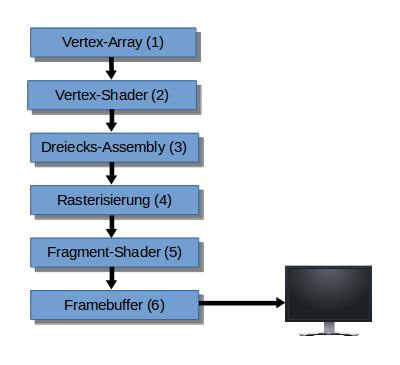
\includegraphics[width=5.2cm]{img/graphics_pipeline.jpg}
	\caption{WebGL Graphik Pipeline}
	\label{fig:webgl_graphics_pipeline}
\end{figure}

Zum \Rd{r}\R{R}endern einer Grafik mit der WebGL Grafik Pipeline werden Arrays von Punkten, welche meist die Ecken eines Dreiecks bilden, in einen Vektorbuffer geschrieben.
Diese werden anschließend vom Vertex-Shader verarbeitet, welcher zum Beispiel Skalierung, Rotation oder Transformation auf die Geometrien anwendet oder Farbinfomation hinzufügt.
Anschließend werden aus den Punkten Dreiecke generiert und in der Rasterisierung die Pixel der Dreiecke berechnet.
Die Pixel bekommen dann vom Fragment-Shader ihre Farbe, welcher diese aus Farbinformationen oder aus zuvor übergebenen Textur-Daten generiert.
Nach der Durchführung eines Tiefentests, 
in welchen überprüft wird welche Pixel sichtbar sind und welche von anderen verdeckt werden bzw der Mischung der Farben bei Transparenz, 
werden die Bildinformationen in den Framebuffer geschrieben,
von wo aus Sie auf dem Bildschirm angezeigt werden können \cite{webgl-introduction}.


%----------------------------------------------
% ** PixiJS 
%----------------------------------------------
\subsubsection{PixiJS}
\label{sec:PixiJS}
Da WebGL eine relativ Hardware nahe API ist wurden einige Frameworks entwickelt welche von der Komplexität einer solchen API abstrahieren, zu denen auch PixiJS zählt.
\Rd{Dies}\R{Es} bietet Funktionen zum Zeichen von \Rd{G}\R{g}eometrischen Figuren, Füllen von diesen und Laden von Texturen.
Eine Szene in PixiJS ist als Baum organisiert\R{,} wobei jeder Knoten in dem Baum wiederum Operationen zur Manipulation wie Transformation, Translation oder Transparenz anbietet.
Ein weiteres Feature ist\R{,} dass auf einen Knoten ein Filter mit WebGL Fragment-Shader-Code gesetzt werden kann\R{,} welcher zur Manipulation der Farbinformation in den einzelnen Bildpunkte dient \cite{pixijs}.

\Rc{bitte lass am besten immer von wem 2ten korrekturlesen - der inhalt is eh wunderbar!}

%----------------------------------------------
% * Funktionalität und Aufbau der Benutzeroberfläche
%----------------------------------------------
\subsection{Funktionalität und Aufbau der Benutzeroberfläche}
\label{sec:Funktionalität und Aufbau der Benutzeroberfläche}
Der Workflow beim Durchsuchen von radiologischen Aufnahmen mit KRESHMOI gliedert sich in folgende Schritte:
\begin{enumerate}
	\item Auswahl eines Start-Datensatzes.
	\item Betrachten des Datensatzes inklusive Fenstern und Zoomen.
	\item Anotieren einer oder mehrerer ROI(s) und eventuelle Eingabe von Text in die Suchzeile.
	\item Suche absenden und Ergebnisse listen.
	\item Betrachen von Datensätzen aus der Ergebnisliste.
	\item Um neue Suchanfrage von ein Ergebnissdatensatz aus zu stellen werden die Schritte von 3 an wiederholt.
\end{enumerate}
Entsprechend dieses Ablaufs wird beim Start der Applikation eine Liste mit allen Datensätzen geladen, 
aus welchen einer als Einstiegspunkt in die Suche ausgewählt werden kann.
Dieser Datensatz wird in den Betrachter der Haupansicht \ref{fig:omip_aplication_layout} geladen.
Die Haupansicht setzt sich aus verschiedenen Interaktions-Elementen (Views) zusammen,
welchen in mehreren möglichen Layouts mit unterschiedlicher Multiplizität und Anordnung miteinander kombiniert werden.
Von diesen Elementen gibt es Vier verschiedene Typen:
\begin{itemize}
	\item Betrachtungsansicht für Volumes (2D-Betrachter)
	\item Betrachtungsansicht für den Report (Report-Betrachter)
	\item Präsentationsansicht für die Ergebnisse (Ergebnis-Liste)
	\item Eingabezeile für Schlagwörter mit dem Suchbutton (Suchzeile)
\end{itemize}
Die Fläche welchen die einzelnen Views innerhalb des Browserfensters einnehmen kann zwischen den Views beliebig verschoben werden, 
unter der Prämisse dass die Bedienelemente der einzelnen Views genügend Platz haben.
Auf den Funktionsumfang des 2D-Betrachters und der Ergebnis-Liste wird in den folgenden Unterkapiteln etwas genauer eingegangen.
\begin{figure}[t]
	\centering
		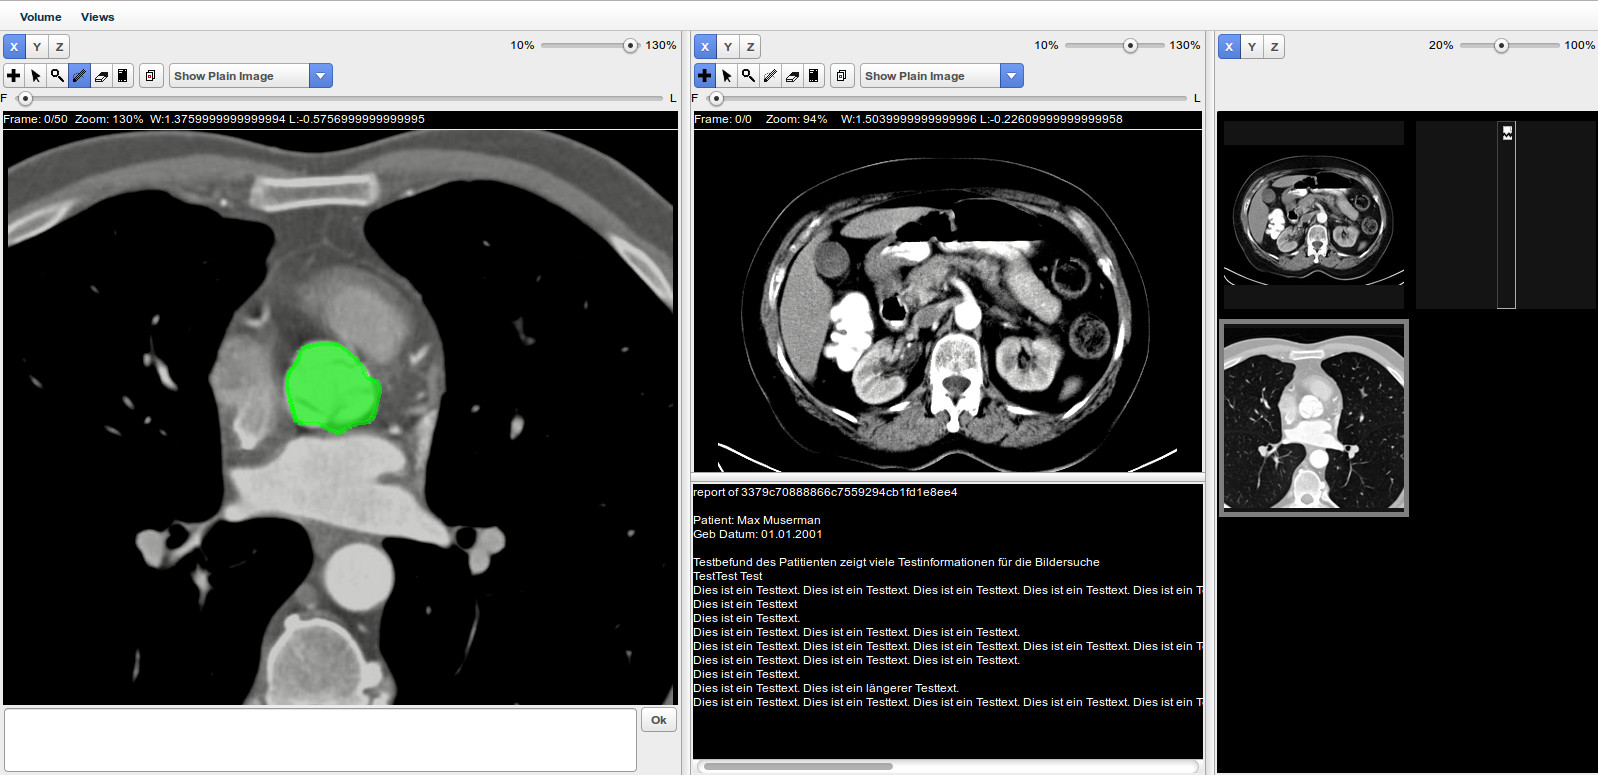
\includegraphics[width=0.8\linewidth]{img/c3_application_standard.jpg}
	\caption{Hauptansicht mit Layout für zwei 2D-Betrachter, Report-Betrachter und Ergebnis-Liste}
	\label{fig:omip_aplication_layout}
\end{figure}


%----------------------------------------------
% ** Funktionalität des 2D-Betrachters
%----------------------------------------------
\subsubsection{Funktionalität des 2D-Betrachters}
\label{sec:Funktionalität des 2D-Betrachters}
Der 2D-Betrachter orientiert sich von seinen Funktionen sehr stark an der Betrachtungssoftware einer PACS-Workstaion oder eines DICOM-Betrachters.
Er ermöglicht die räumliche Navigation durch die Schnitte eines Volumes in einer bestimmten Orientierung, sowie das Umschalten zwischen den Orientierungen.
Des weiteren kann wenn das Volume aus der Ergebnissliste einer Suche ausgewählt wurde, 
also nicht der Startdatensatz ist,
eine Anzeige mit den Deckungsbereichen der Suche hinzu geschaltet werden. 

Zur Interaktion mit den Volume wird auch wie bei anderen Betrachtern der Maus eine bestimmte Funktion zugewiesen.
Die Funktionen umfassen Fensterung, Zoom, Bewegen des Bildes und Zeichnen und Löschen von Polygonen (ROIs).
Das Einzeichnen von ROIs ist um die Benutzung einfach zu halten auf ein einzelnes Schnittbild beschränkt.
Wird das Werkzeug zum Zeichen oder Löschen von Polygonen auf mehreren Schnitten verwendet springt der Betrachte bei deren Aktivierung immer wieder auf das Schnittbild mit dem ersten Polygon zurück.
Das Bild kann halb Transparent mit dem Report des Datensatzes überblendet werden, was aber die Mausfunktion auf das Scrollen des Reports reduziert.
In allen anderen Funktionen ist das Scrollen immer an die Navigation durch die Schnitte gebunden.

%----------------------------------------------
% ** Funktionalität der Ergebniss-Liste
%----------------------------------------------
\subsubsection{Funktionalität der Ergebniss-Liste}
\label{sec:Funktionalität der Ergebniss-Liste}
Die Ergebnis-Liste präsentiert die Ergebnisse einer Suche welches sie über Drag and Drop in einen Betrachter laden lassen.
Die Präsentation erfolgt über ein Vorschaubild welches von KRESHMOI als repräsentatives Bild für die Suche gewählt wurde.
Um ein Suchergebniss im Vorfeld zu Beurteilen verfügt die Ergebnis-List ebenfalls über die Funktion die Orientierung der Schnitte des Volumes zu ändern und die Vorschaubilder zu zoomen.

%----------------------------------------------
% * Technische Umsetzung
%----------------------------------------------
\subsection{Technische Umsetzung}
\label{sec:Technische Umsetzung}
In dem Unterkapitel Technische Umsetzung wird im Groben die Archtiktur der Applikation sowie von komplexeren Komponenten erklärt und auf wichtige Details bei deren Umsetzung eingegangen.
Weiters wird angegeben wie die Fensterung mit zwei verschidenen Technologie implementiert wurde.

%----------------------------------------------
% ** Umsetzung der dynamischen Layouts
%----------------------------------------------
\subsubsection{Framework für dynamischen Layouts}
\label{sec:Umsetzung der dynamischen Layouts}

%----------------------------------------------
% ** Berehnung der Fensterung
%----------------------------------------------
\subsubsection{Berehnung der Fensterung}
\label{sec:Berehnung der Fensterung}
Die Berechnung der Fensterung ist eine Anpassung von Kontrast und Helligkeit des Bildes,
wozu für jedes Pixel der Farbwert mit einer Linear Transformation in einen neuen Zielwert überführt werden muss.
\begin{equation}
        F(x) = c*x + b
\end{equation}
Dabei ist der Kontrast durch $c$ und die Helligkeit durch $b$ gegeben.
Für diese Berechnung wurde ein Ansatz auf Basis von JavaScript durch die Canvas 2D API und eine Implementierung mit Web GL getestet.

\paragraph{Canvas 2D API}
Für die graphische Ausgabe im Browser wird ein HTML5 Canvas Element verwendet,
auf welches über ein sogenanten Grafikkontext zugegriffen werden kann. 
Dieser Grafikkontext wird in JavaScript vom Browser als Objekt zur Verfügung gestellt.
Durch das Kontext-Objekt kann der Bildinhalt in ein Array von Farbwerten und umgekehrt auch ein Array von Farbwerten in das Bild geschrieben werden.
Dabei wird das Bild zeilenweise in ein eindimensionales Array Serialisiert, 
wo jeder Bildpunkt auf 4 Speicherstellen mit einem Integer-Wert zwischen 0 und 255 abgebildet wird.
Die ersten drei Speicherstellen bilden den Farbwert durch die Anteile von Rot, Grün, Blau und die vierte den Alpha Kanal.
Für die Fensterung müssen alle Speicherstellen für die Farbe transformiert und wieder auf einen Integer Wert gerundet werden.
%
Um unnötige Berechnungen für jedes einzelne Pixel zu sparen, werden pro Fensterungsschritt alle Pixelwerte zwischen 0 und 255 einmal vor berechnet und in einer LookUp Tabelle als Array gespeichert.
Anstatt den Wert für jedes Pixel neu zu berechen und zu runden fungiert bei diesem Ansatz der aktuelle Wert eines Pixels als Schlüssel für die Tabelle welche den neuen Wert des Pixels enthält.
Die Anzahl der Operationen wird dabei auf 255 Berechnungen und die Anzahl der Speicherzugriffe pro Bildpunkt sowie die der LookUp Tabelle reduziert.
\begin{figure}[t]
\begin{lstlisting}[
	language=JavaScript,
	firstnumber=1,
	caption=Ändern von Kontrast und Helligkeit in einem HTML Canvas Element mit einer LookUp Tabelle in JavaScript
]
function calcWindowForDomElement(domElement, contrast, brightness)
{
    var ctx = domElement.getContext("2d");
    var w = domElement.width;
    var h = domElement.height;

    var lut = getLookUpTable(contrast, brightness);
    var image = ctx.getImageData(0, 0, w, h);
    var imageData = image.data;
    var imageDataSize = (w * h * 4);

    for(var pos = 0; pos < imageDataSize; pos = pos + 4){
        imageData[pos] = lut[imageData[pos]];
        imageData[pos + 1] = lut[imageData[pos + 1]];
        imageData[pos + 2] = lut[imageData[pos + 2]];
    }

    ctx.putImageData(image,0,0);
}
\end{lstlisting}
\end{figure}
%
\begin{figure}[t]
\begin{lstlisting}[
	language=JavaScript,
	firstnumber=1,
	caption=Berechnung der LookUp Tabelle
]
function getLookUpTable(contrast, brightness){
    var lut = new Array();

    for(var i = 0; i < 256; i++){
        var newVal = Math.round(contrast * i + brightness);
        if(newVal < 0) newVal = 0;
        if(newVal > 255) newVal = 255;
        lut[i] = newVal;
    }

    return lut;
}
\end{lstlisting}
\end{figure}

\paragraph{WebGL}
Die Berechnung der Fensterung in der WebGL Grafik Pipeline erfolgt im Fragment-Shader.
Dazu wird über die WebGL-API zuerst ein Array von Punkten, 
welches die Grundfläche in der Form von zwei aneinander liegenden Dreiecken darstellt übergeben.
Weiters wird das Bild für die Fensterung als Textur in den Speicher der Grafikkarte geladen und die Variablen für Helligkeit und Kontrast übergeben.
Der Vertex-Shader fügt den Punkten einen Vektor mit Textur-Koordinaten hinzu, welche an den Fragment-Shader weitergereicht werden.
Dieser kann dann mit Hilfe der Textur-Koordinaten für jedes Pixel der Grundfläche die Farbe des Pixels aus der gepufferten Textur laden.
Die Repräsentation der Farbe erfolgt mit dem Datentyp $vec4$ welcher eine Vierdimensionalen Vektor für Fließkommazahlen darstellt.
Die ersten Drei Dimensionen bilden die Drei Grundfarbe Rot, Grün, Blau die vierte den Alpha-Kanal, welche jeweils von einem Wert zwischen 0 und 1 repräsentiert werden.
Bevor die Farb-Information des Pixels zurückgegeben wird erfolgt die Fensterung durch einen Linear-Transformation auf die drei Farbkanäle des Farbvektors.
Die Rückgabe der Farbinformation erfolgt durch das ablegen in der Variable $gl\_FragColor$.
\begin{figure}[t]
\begin{lstlisting}[
	language=GLSL,
	firstnumber=1,
]
precision mediump float;

uniform sampler2D u_image;
varying vec2 vTextureCoord;

uniform float contrast;
uniform float brightness;

void main() {
    vec4 color = texture2D(u_image, vTextureCoord);
    gl_FragColor.r = color.r * contrast + brightness;
    gl_FragColor.g = color.g * contrast + brightness;
    gl_FragColor.b = color.b * contrast + brightness;
    gl_FragColor.a = color.a;
}
\end{lstlisting}
\caption{Fragment-Shader-Code zum Rendern und Fenstern der Slices}
\end{figure}


%----------------------------------------------
% ** 2D Betrachter
%----------------------------------------------
\subsubsection{2D Betrachter}
\label{sec:2D Betrachter}
Für die Implementierung des 2D-Betrachters wurde neben Cappuccino für die Bedienelemente auch noch Pixi.JS für das Grafikfenster zur Darstellung des Volumes verwendet.
Der Inhalt des Grafikfensters ergibt sich aus den inhalt von mehreren übereinanderliegenden Layern.
\begin{itemize}
	\item \textbf{ImageLayer} zur Darstellung der Schnitte des Volumes
	\item \textbf{AnotationLayer} zum zeichnen der ROIs
	\item \textbf{ZoomLayer} zur Darstellung des Zoom-Rechecks
	\item \textbf{ReportLayer} zum Render des Berichtes in das Bild
\end{itemize}
Bei diesen Layern werden Skalierung und Positionierung nur auf den ImageLayer und den AnotationLayer angewendet, die anderen füllen jeweils nur das ganze Grafikfenster aus.
Um die Software möglichst erweiterbar zu gestalten,
wurde eine LayerKlasse $PixiLayer$ entwickelt welcher eine beliebige Menge von Sublayern hizugefügt werden kann.
Dabei wird zwischen statischen Sublayern welche jeweils nur die Anzeigefläche ausfüllen und dynamischen Sublayern welche gemeinsam skaliert und positioniert werden können unterschieden.
Diese Layerklasse erledigt auch die konvertierung von Punkten zwischen den dynamischen und den statischen Sublayern, in Hisicht auf Postion, Skalierung und Layerdimension.
Da die restliche GUI mit Cappuccino aufgebaut wurde und dieses Framework auch die Ereignisse für Größenänderungen der einzelen Views behandelt,
müssen diese vom ViewObjekt welches den 2D-Betrachter Kapselt an das Grafikfenster weiter gegeben werden.
Ansonsten ist das Pixi.JS basierte Grafikfenster durch die LayerKlassen bis auf Funktionen zur Übergabe der Anzeigedaten und zur Punktkonvertierung vom 2D-Betrachter abgeschottet.
Die eigentliche Logik des Betrachters ist in den Layern zugeordnete Controller-Klassen gekapselt.
Die Betrachter-Klasse selbst ist hauptsächlich für die Erstelltung der Bedienelemente und die Behandlung von Events verantwortlich.
\begin{figure}[t]
	\centering
		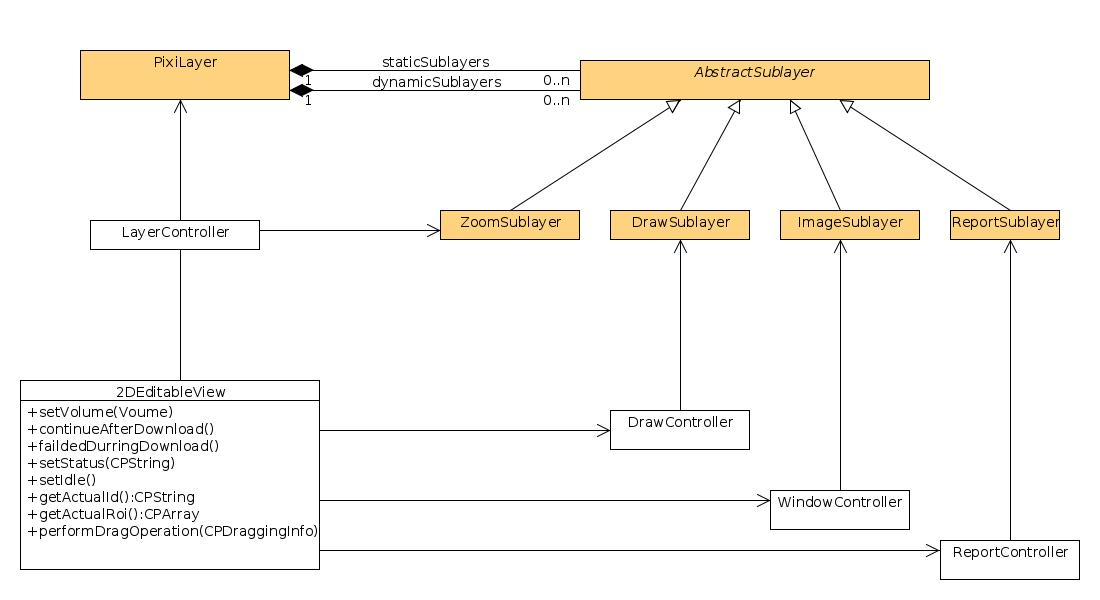
\includegraphics[width=\linewidth]{img/s3_2dview_class_structure.jpg}
	\caption{Struktur des 2D-Betrachters als Klassendiagramm}
	\label{fig:omip_aplication_layout}
\end{figure}

%----------------------------------------------
% * Kommunikation mit KRESHMOI
%----------------------------------------------
\subsection{Kommunikation mit KRESHMOI}
\label{sec:Kommunikation mit KRESHMOI}
Der Datenaustausch mit KRESHMOI basiert auf REST wobei sowohl auf die einzelnen Slices von einem Volume, als auch auf die Suche als Ressource über eine URL zugegriffen werden kann.

%----------------------------------------------
% ** Query nach Bilderns
%----------------------------------------------
\subsubsection{Query nach Bildern}
\label{sec:Query nach Bildern}
Der Zugriff auf die Suchfunktion erfolgt über eine POST-Operation in welcher die Anfrage und die Antwort in JSON codiert werden.
Zum Ausführen einer Suchanfrage stehen zwei Ressourcen zur Verfügung:
\\
\\
\textit{/index}\\
Liefert ein Array von allen Verfügbaren Datensätzen zurück 
\\
\\
\textit{/query}\\
Liefert ein Array von Datensätzen zurück welche anhand der Übergebenen Suchkriterien gefunden wurden.
Eine Suchanfrage basiert immer auf einen Datensatz welcher in der Anfrage übergeben werden muss.
In diesem Datensatz werden weiters Interessante Bereiche sogenannte ROIs (Region of Interesst) in den einzelnen Schnittbildern definiert.
Die Übergabe einer ROI erfolgt als Polygon in Form einer Listen von Punkten im Dreidimensionalen Raum des Volumes.
\begin{figure}[t]
\begin{lstlisting}[
	language=json,
	firstnumber=1,
	caption=Query
]
{
   "queryid":"",
   "text":"",
   "imageid":"",
   "roi": 
   [
      "polygon":
      [
         "point":{"x":0, "y":1, "z":0},
         "point":{"x":1, "y":1, "z":0},
         "point":{"x":0, "y":0, "z":0}
      ],

   ]
}
\end{lstlisting}
\end{figure}


\begin{figure}[t]
\begin{lstlisting}[
	language=json,
	firstnumber=1,
	caption=Result
]
{
   "rankedImageID": 
   [
      {
         "imageID": "9587336b132b127b936ad0afd80ca862",
         "normalDimX": 52,
         "normalDimY": 512,
         "normalDimZ": 512,
         "relevance": 1,
         "report": "",
         "title": "Some Image"
      },
   ]
}
\end{lstlisting}
\end{figure}

%----------------------------------------------
% ** Laden der Bilder
%----------------------------------------------
\subsubsection{Laden der Bilder}
\label{sec:Laden der Bilder}
Die Bilddaten eines Volumes können über eine GET-Operation geladen werden.
Dabei wird jedes Volume als eine Resource im Unterverzeichnis \textit{/image/} identifiziert.
Über Parameter in der URL werden die Schnittrichtung und und die Nummer des Bildes in der jeweiligen Schnittebene angegeben.
Wir keine Nummer für das Bild angegeben wählt KRESHMOI eine repräsentatives Bild für die Suchanfrage, welches für die Präsentation der Ergebnisse verwendet wird.
Für die Schnittebene gibt es entsprechende der Terminologie für die Bildgebung in der Anatomie die Optionen:
\begin{itemize}
	\item Axial: Die Schnitte erfolgen Waagrecht in der Transversalebene
	\item Sagital: Die Schnitte erfolgen Senkrecht in der Sagitalebene
	\item Coronal: Die Schnitte erfolgen Senkrecht in der Frontalebene 
\end{itemize}
Sollen die Regionen welche der Suchanfrage entsprechen in den einzelnen Bildern markiert werden, muss die Query-ID mit übergeben werden um die ursprüngliche Suchanfrage zu identifizieren.
\\
\\
Beispiel:
\\
\url{/image/9587336b132b127b936ad0afd80ca86.jpg?slice=1&direction=axial&query=1}
%TODO: Prüfen ob URL ok
%TODO: Zitieren von KRESHMOI API
%TODO: Zitieren der Schnittebenen
%TODO: Bild ist wikipedia ok: http://de.wikipedia.org/wiki/Anatomische_Lage-_und_Richtungsbezeichnungen

%!TEX root = cvl_bachelor_thesis.tex

%-------------------------------------------------------
% Results
%-------------------------------------------------------
\section{Results}
\label{sec:results}

%----------------------------------------------
% * Geschwindigkeit 
%----------------------------------------------
\subsection{Performance}
\label{sec:Performance}

In Absatz \ref{sec:Berehnung_der_Fensterung} wurden zwei Ansätze zur Berechnung der Fensterung vorgestellt,
welche jeweils auf unterschiedlichen vom Browser zur Verfügung gestellten API's basieren.
In diesem Unterkapitel wird gezeigt, wie sich diese beiden Verfahren im Bezug auf ihre Performance verhalten.
Dazu wird ein Testsystem vorgestellt, mit dem diese gemessen wurde und weiters werden die Ergebnisse dieser Messungen präsentiert und diskutiert.

\subsubsection{Messverfahren}
Um zu evaluieren wie performant ein Verfahren ist,
wurde über einen bestimmten Zeitraum $T_m$ ermittelt, wie viele Bilder durchschnittlich in der Sekunde berechnet werden können.
Dieser Wert wird als Framerate bezeichnet und in FPS (Frames per Second) angegeben.
Die Framerate ist von folgenden Faktoren abhängig:
\begin{itemize}
	\item Berechnungs-Verfahren
	\item Anzahl der Pixel im Bild
	\item Verwendete Hardware
	\item Verwendeter Browser
	\item Aktuelle Auslastung der Maschine
\end{itemize}
Die ersten vier Parameter wurden für die verschiedenen Messungen variiert, während der letzte eine Störgröße darstellt, welche nur bedingt beeinflusst und nicht absolut konstant gehalten werden kann.
Bei jeder Messung wurden die durchschnittlichen FPS in Abhängigkeit von der Bildgröße aufgenommen.
Eine Messung besteht daher aus einer Menge von Messpunkten, wobei jeder die durchschnittliche Framerate für eine bestimmte Bildgröße angibt.
Dabei wurde ein quadratisches Bild verwendet und dessen Kantenlänge zwischen zwei Messpunkten jeweils um einen bestimmten Wert $\Delta_{edge}$ vergrößert.
Die Pixelanzahl zwischen zwei Messpunkten hat somit ein quadratisches Wachstum wie es auch beim Zoomen von Bildern in der Applikation der Fall ist.

Für die Durchführung der Messung wurde eine eigene Messumgebung entwickelt, 
mit welcher es möglich ist die Implementierung der beiden Verfahren mit unterschiedlichen Parametern zu testen.
Die Messumgebung besteht aus einem Servlet welches mit Spring MVC implementiert wurde und aus einer Clientseitigen Testumgebung für die Implementierungen der beiden Verfahren.
Eine Messung wird durch den Aufruf einer Resource auf dem Servlet gestartet und parametriert.
Das Servlet retourniert darauf hin eine Webseite in welcher die Testumgebung als JavaScript ausgeführt wird.
Diese versucht auf einem Bild die Fensterung mit einer Ziel-Framerate von 60FPS zu berechnen und misst Abfälle in der Framerate.
Für die eigentliche Messung wurde das Tool Stats.JS verwendet und geringfügig modifiziert um die gemessenen Werte auslesen zu können.
Nach Ablauf der Messzeit $T_m$ werden die gemessenen Werte zurück an den Server gesendet, welcher diese in eine Datenbank schreibt.
Der Server antwortet darauf mit einem neuen Messpunkt wobei das Testbild zwischen den Messpunkten jedes mal um den Wert $\Delta_{edge}$ vergrößert wird, 
bis es eine vorher festgelegte maximale Bildgröße ereicht hat.

\subsubsection{Ergebnisse}
Im letzten Unterkapitel wurde ein Verfahren zur Ermittlung der Framerate in Abhängigkeit von der Bildgröße vorgestellt, 
sowie mehrere Parameter welche auf diese Größe einen Einfluss haben.
Von diesen Parametern wurden die Hardware \ref{tab:tested_hardware}, 
der Browser \ref{tab:tested_browser} und das Verfahren zum Rendern \ref{tab:tested_technologies} in unterschiedlichen Kombinationen getestet und einen Kennline ermittelt.
\begin{figure}[t]
	\centering
	\begin{tabular}{| l | l | l |}
		\hline
				& PC				& Tablet \\
		\hline
		Prozessor	& Intel Core i7-2600K 3.40GHz	& Nvidia Tegra 3 1.30GHz \\
		Arbeitsspeicher	& 12GB DDR3-1333		& 1GB DDR3-1333 \\
		Grafikkarte	& Nvidia GeForce 8800 GTS	& Nvidia GeForce ULP \\
		GPU Kerne	& 96				& 12 \\
		Grafikspeicher	& 640MB 800 MHz			& Shared mit CPU \\
		Betriebssystem	& Windows 8			& Android 4.4.4 \\
		\hline
	\end{tabular}
	\caption{Harware-Konfiguration der geteseten Geräte}
	\label{tab:tested_hardware}
\end{figure}
\begin{figure}[t]
	\centering
	\begin{tabular}{| l | l |}
		\hline
		Browser			& Version \\
		\hline
		Chrome			& 39.0 \\
		Chrome for Android 	& 39.0 \\
		FireFox			& 34.0.5 \\
		InternetExplorer	& 11.0 \\
		Opera			& 26.0 \\
		Safari			& 5.1.7 \\
		\hline
	\end{tabular}
	\caption{Getestete Browser}
	\label{tab:tested_browser}
\end{figure}
\begin{figure}[t]
	\centering
	\begin{tabular}{| l | l |}
		\hline
		Verfahren	& Verwendete Technologien \\
		\hline
		WebGL		& Canvas3D API, Pixi.JS, JavaScript \\
		Canvas 2D	& Canvas2D API, JavaScript \\
		\hline
	\end{tabular}
	\caption{Getestete Verfahren mit verwendeten Technologien}
	\label{tab:tested_technologies}
\end{figure}


Die Abbildungen \ref{fig:stat_renderer_pc_chorme} und \ref{fig:stat_renderer_tablet_chorme} zeigen einen Vergleich der beiden rendering Verfahren auf jeweils unterschiedlicher Hardware mit Chrome.
In beiden Fällen verhält sich WebGl wesentlich performanter als das Rendering der Bilder in der CPU.
Am PC mit einer Grafikkarte aus dem Jahr 2007 wurden Bilder bis zu 3000Pixel Kantelänge getestet, 
welche sich ohne Einbrüche mit 60FPS render liesen.
Dieses Verhalten lässt sich dadurch erklären dass eine GPU für diese Anwendung wesentlich geeigneter ist.
Zu den beschleunigenden Faktoren zählen unter anderem, das Zusammenarbeiten vieler paralleler Shader-Kerne welche selbst wiederum sehr stark für diese Art von Berechnungen optimiert sind.
Weitere Faktoren sind die schnelle Anbindung des Grafikspeichers in dem das Bild als Textur abgelegt wird, und dass die GPU auf weniger parallele Prozesse aufgeteilt wird als die CPU.
Am PC wurden dieses Tests auch mit anderen Browsern durchgeführt welche hier nicht abgebildet sind, da die Ergebnisse sehr ähnlich waren.

Unterschiede zwischen den verschiedenen Browsern zeigten sich nur beim Rendern mit Canvas 2D was in Abbildung \ref{fig:stat_browser_js_pc} dargestellt wird.
Bei dieser Gegenüberstellung wird die Performance ausschließlich durch die Implementierung des Browsers bestimmt,
wobei hier die Effizienz der JavaScript-Engine am meisten Einfluss hat.
Bei diesen Test ist noch anzumerken dass nicht davon ausgegangen werden kann, 
dass die JavaScript Interpreter für diese Art von Operationen, 
also dem verarbeiten von großen linearen Daten-Arrays optimiert wurden, 
da diese Art der Datenverarbeitung in klassischen Html5 Anwendungen eher selten vorkommt.
Das unterschiedliche Verhalten der Browser mit WebGl wurde hier nicht dargestellt da die Performance bis zu einer Größe von 3000Pixel Kantenlänge bei allen Browsern konstant 60FPS beträgt.
Die einzige Ausnahme bildet der Browser Safari in welchen WebGl nur experimentell verfügbar ist und extra aktiviert werden muss, was in der getesteten Version nicht möglich war.
Es ist auch anzunehmen dass beim Rendern mit WebGl der Browser selbst keine nennenswerte Rolle spielt da die Datenverarbeitung in der GPU passiert und der Browser nur das Ergebnis darstellt.

In den Abbildungen \ref{fig:stat_hardware_js_chrome} und \ref{fig:stat_hardware_webgl_chrome} wird die Performance auf unterschiedlicher Hardware gezeigt.
Obwohl sich beim Browser Chrome die Tablet Version in einigen Features von der Desktop Version unterscheidet, 
ist anzunehmen dass Dies auf die Performance keine Auswirkung hat da sie beide die selbe JavaScript Engine verwenden.
Die Unterschiede in der Leistung beim Rendern mit Canvas 2D erklärt sich durch die wesentlich geringere Leistung der CPU im Tablet gegenüber dem PC.
Beim Rendern mit WegGl führt die schwächere GPU des Tablets zu der schlechteren Performance.

\begin{figure}[pt]
	\centering
	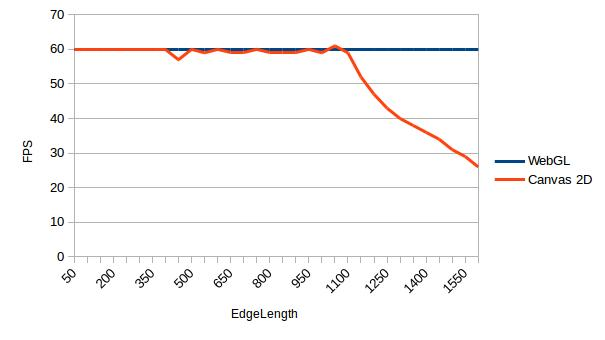
\includegraphics[width=0.7\linewidth]{img/c4_stat_renderer_pc_chorme.jpg}
	\caption{Performance unterschiedlicher rendering Verfahren am PC mit Chrome}
	\label{fig:stat_renderer_pc_chorme}
\end{figure}

\begin{figure}[pt]
	\centering
	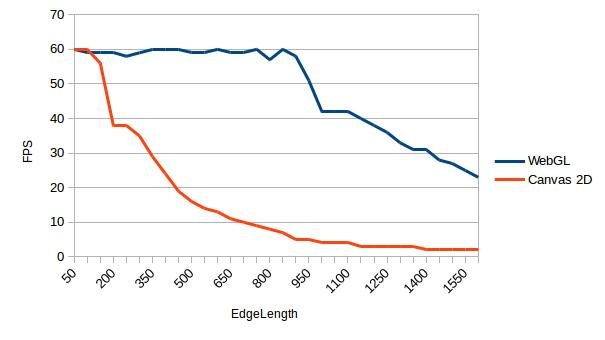
\includegraphics[width=0.7\linewidth]{img/c4_stat_renderer_tablet_chorme.jpg}
	\caption{Performance unterschiedliche rendering Verfahren am Tablet mit Chrome}
	\label{fig:stat_renderer_tablet_chorme}
\end{figure}

\begin{figure}[pt]
	\centering
	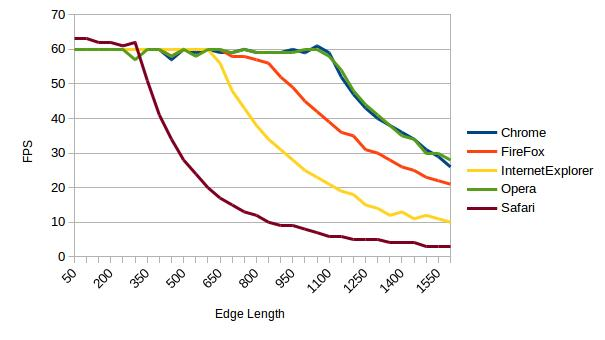
\includegraphics[width=0.7\linewidth]{img/c4_stat_browser_js_pc.jpg}
	\caption{Performance unterschiedlicher Browser beim Rendering mit Canvas 2D}
	\label{fig:stat_browser_js_pc}
\end{figure}

\begin{figure}[pt]
	\centering
	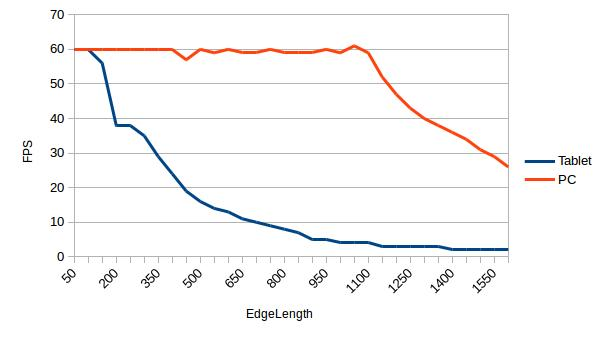
\includegraphics[width=0.7\linewidth]{img/c4_stat_hardware_js_chrome.jpg}
	\caption{Performance unterschiedlicher Hardware mit Canvas 2D in Chrome}
	\label{fig:stat_hardware_js_chrome}
\end{figure}

\begin{figure}[pt]
	\centering
	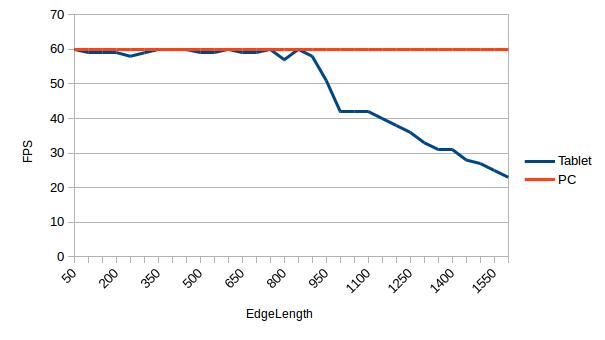
\includegraphics[width=0.7\linewidth]{img/c4_stat_hardware_webgl_chrome.jpg}
	\caption{Performance unterschiedlicher Hardware mit WebGL in Chrome}
	\label{fig:stat_hardware_webgl_chrome}
\end{figure}

\subsubsection{Zusammenfassug der Ergebnisse}
Im letzten Unterkapitel wurden Messergebnisse für die Performance in Abhängigkeit von Rendering-Verfahren, Hardware und Browser gezeigt.
Zusammenfassen lässt sich sagen, 
dass unter der Verwendung von WebGl auf einem aktuellen PC, 
Bilder bis zu einer Auflösung von 9 MegaPixel problemlos fenstern lassen.
Auf dem verwendeten Tablet liegt die Grenze bei ca einem MegaPixel.
Rendern mit Canvas 2D liefert im Vergleich zu WebGl wesentlich schlechtere Performance und lässt sich in der Praxis am Tablet nicht sinnvoll verwenden.


%----------------------------------------------
% * Usability
%----------------------------------------------
\subsection{Vergleich mit dem KRESHMOI JavaClient}
\label{sec:Usability}
In der Einführung wurde bereits erwähnt, 
dass für KRESHMOI paralell zu der in diesem Projekt entwickelten Webapplikation auch noch ein Radiologie-Client in Java entwickelt wurde.
Wie auch die Webapplikation dient der JavaClient zum Betrachten und Durchsuchen von radiologischen Bilddaten,
bietet aber weiters noch umfangreiche Tools für die Textsuche und für kolaboratives Arbeiten.
In diesem Unterkapitel werden Features und die Umsetzung der beiden Anwendung bezüglich des Pflichtenheftes (Siehe Unterkapitel \ref{sec:Pflichtenheft}) verglichen.



%!TEX root = cvl_bachelor_thesis.tex

%-------------------------------------------------------
% Conclusion
%-------------------------------------------------------
\section{Conclusion}
\label{sec:conclusion}
In dieser Arbeit wurde die Umsetzung eines Browser basierten Frontend's für einer Suchmaschiene für radiologische Bilddaten gezeigt.
Es wurde anhand von zwei gängigen Software-Produkten zur Betrachtung von radiologischen Bilddaten die wichtigsten Anforderungen analysiert und mit der Erweiterung um die Suchfunktion als Webapplikation umgesetzt.
Es wurde gezeigt dass es mit den aktuell verfügbaren Technologien und Frameworks ohne Probleme möglich ist eine Betrachter für radiologische Bilddaten für den Browser zu implementieren.



% bibliography
\addcontentsline{toc}{section}{Bibliography}
\bibliographystyle{alpha}
\bibliography{cvl_tr.bib}

\end{document}

